% Optimal binary search tree (generated by figs_c2ch05.py).
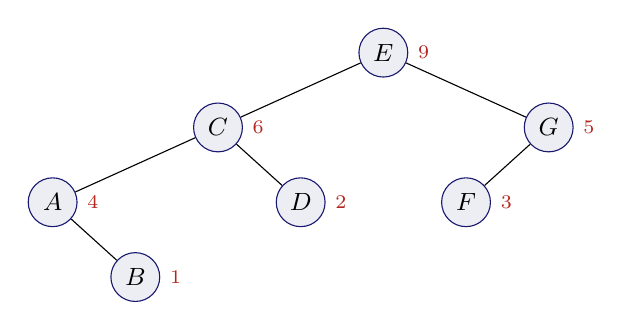
\begin{tikzpicture}[x=1.05cm,y=0.95cm,every node/.style={font=\small}]
\tikzset{nd/.style={circle,draw=MidnightBlue,fill=MidnightBlue!8,inner sep=1pt,minimum size=0.62cm}}
\node[nd] (k5) at (5,0) {$E$};
\node[font=\scriptsize,BrickRed,right=0pt] at (k5.east) {9};
\node[nd] (k3) at (3,-1) {$C$};
\node[font=\scriptsize,BrickRed,right=0pt] at (k3.east) {6};
\node[nd] (k1) at (1,-2) {$A$};
\node[font=\scriptsize,BrickRed,right=0pt] at (k1.east) {4};
\node[nd] (k2) at (2,-3) {$B$};
\node[font=\scriptsize,BrickRed,right=0pt] at (k2.east) {1};
\node[nd] (k4) at (4,-2) {$D$};
\node[font=\scriptsize,BrickRed,right=0pt] at (k4.east) {2};
\node[nd] (k7) at (7,-1) {$G$};
\node[font=\scriptsize,BrickRed,right=0pt] at (k7.east) {5};
\node[nd] (k6) at (6,-2) {$F$};
\node[font=\scriptsize,BrickRed,right=0pt] at (k6.east) {3};
\draw (k5) -- (k3);
\draw (k3) -- (k1);
\draw (k1) -- (k2);
\draw (k3) -- (k4);
\draw (k5) -- (k7);
\draw (k7) -- (k6);
\end{tikzpicture}
